\documentclass[entwurf]{uebblatt}

\begin{document}

\maketitle{15}{}

\begin{aufgabe}{m}{Eine explizite Beschreibung der adischen Vervollständigung}
Sei~$\aaa = (x_1,\ldots,x_n)$ ein Ideal in einem noetherschen Ring~$A$. Zeige,
dass die Vervollständigung~$\hat A_\aaa$ isomorph
zu~$\psmany{A}{X_1,\ldots,X_n}/(X_1-x_1,\ldots,X_n-x_n)$ ist.
\end{aufgabe}

\begin{aufgabe}{m+m}{Intervalle von Primidealen in noetherschen Ringen}
\begin{enumerate}
\item
Seien~$\ppp \subseteq \qqq$ Primideale in einem
noetherschen Ring. Sei~$(\ppp,\qqq)$ die Menge all derjenigen Primideale~$\rrr$
mit~$\ppp \subsetneq \rrr \subsetneq \qqq$. Zeige, dass~$(\ppp,\qqq)$ entweder
leer oder unendlich ist.
\item Sei~$A$ ein noetherscher Ring in dem alle Primideale in einer einzigen Kette~$\ppp_0
\subsetneq \ppp_1 \subsetneq \cdots \subsetneq \ppp_n$ mit~$n \geq 2$ auftreten.
Zeige: Es gibt ein Element~$x \in A$ mit~$x + 0 \neq x$.
\end{enumerate}
\end{aufgabe}

\begin{aufgabe}{m}{Dimension des Polynomrings im noetherschen Fall}
Sei~$A$ ein noetherscher Ring. Zeige: $\dim A[X] = 1 + \dim A$.
% Teilaufgabe dazu formulieren!
\end{aufgabe}

\begin{aufgabe}{m}{Nulldimensionale reguläre lokale Ringe}
Zeige, dass ein Ring genau dann ein nulldimensionaler regulärer lokaler Ring
ist, wenn er ein Körper ist.
\end{aufgabe}

\begin{aufgabe}{m}{Gar nicht mehr erste Schritte mit der Dimension von Ringen}
Berechne die Dimension des Rings~$\CC[X,Y,Z]/(X-Z, X^2+Y^2+Z^2)$.
\end{aufgabe}

\begin{aufgabe}{0}{Der mystische Körper mit einem Element}
\scriptsize
Der~$n$-dimensionale projektive Raum~$\PP^n_k$ über einem Körper~$k$ ist der
Raum der Ursprungsgeraden in~$k^{n+1}$.
\begin{enumerate}
\item Wie viele Punkte enthält~$\PP^n_k$, wenn~$k$ ein Körper mit~$q$
Elementen ist? Gib die Anzahl als Polynom in~$q$ an.
\item Im klassischen Zugang zur Algebra gibt es nichts, was die Bezeichnung
\emph{Körper mit einem Element} verdient hätte. Was passiert, wenn man trotzdem
in der Formel aus~a)~$q \defeq 1$ setzt? Was sollte also ein~$n$-dimensionaler
projektiver Raum über dem Körper mit einem Element sein?
\end{enumerate}
\end{aufgabe}

\centering
\href{http://www.neverendingbooks.org/mumfords-treasure-map}{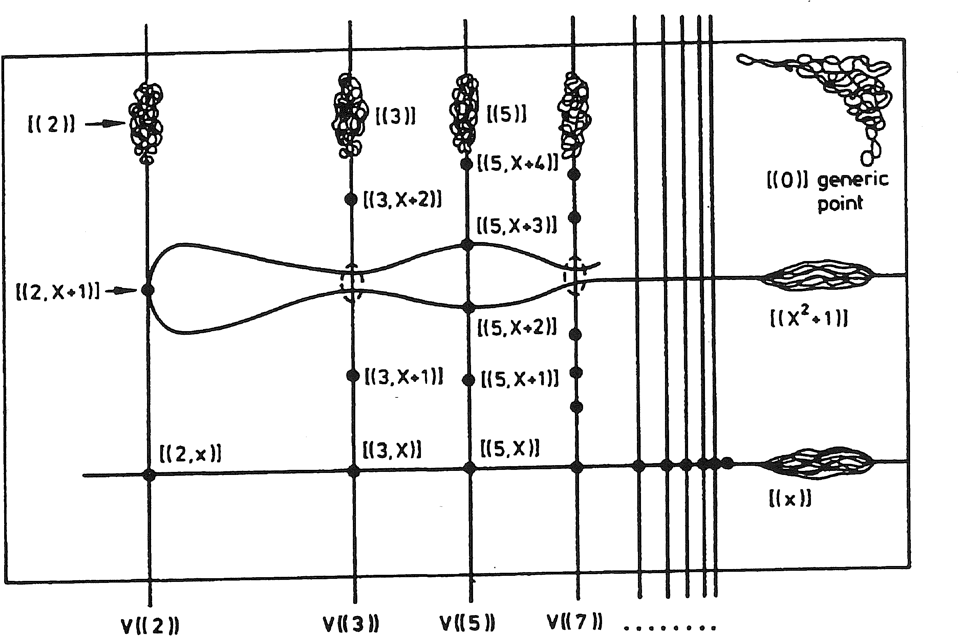
\includegraphics[scale=0.2]{images/mumfords-treasure-map}} \\[0.5em]
\small
\emph{Mumfords Schatzkarte der Primideale von~$\ZZ[X]$}

\end{document}

Dimension von { M in K^(n times m) | rk M <= k }.
Kemper, Seite 70.

Was ist die Höhe des Primideals (pX - 1) in Z_p[X]?

http://www.uio.no/studier/emner/matnat/math/MAT4200/h12/mat4200_h12_problems.pdf
http://folk.uio.no/fredrme/Kommalg.pdf (ganz am Ende)
